%Oppgave 2: Innovasjon og mennesker 


\subsection{Task A}
\subsubsection{Innledning}
Vi har her valgt å ta utgangspunkt i to stillinger fra firmaet Tungesvik Stålesveis. Vi vil først ta for oss og vurdere kvaliteten på jobben som sveiser i Tungesvik Stålesveis, og så vil vi ta for oss jobben Helle Loholt har som økonomisjef. Vi vil sammenligne jobbene deres med de fem hovedelementene som, i følge jobbkarakteristikamodellen, påvirker en arbeidstakers indre motivasjon; ferdighetsvariasjon, oppgaveidentitet, oppgaveviktighet, autonomi og tilbakemelding. Disse faktorene brukes for å anslå motivasjonspotensialet i en jobb, der man kan stille en jobbdiagnose ved å regne ut MPS. Dette har vi gjort i et senere avsnitt.

Tungesvik Stålesveis er en familiebedrift, der flere av arbeiderne er slektninger av gründeren som startet opp bedriften. Sveiserne er plukket ut av Olav Tungesvik, nåværende direktør. Til sammen plukket han ut 18 sveisere, derav 8 som var villige til å gå på kurs i metallbearbeiding

\subsubsection{Sveiserne}
I produksjonsavdelingen, hvor sveiserne jobber, er arbeidet delt inn i små arbeidsoppgaver. Den enkelte arbeider er ekspert på spesielle arbeidsoppgaver. Det vil si at graden av ferdighetsvariasjon er liten. I et intervju betegner en sveiser jobben sin som “innmari kjedelig”. Han sier at “Vi er gått over fra å være håndverkere til å bli fabrikkarbeidere”. Det er klart at jobben blir mindre motiverende når man går fra å ha varierte oppgaver innen båtbygging til å kun være ekspert på å f.eks. sveise sammen to metallbiter.

Under produksjon av individuelle deler har sveiserne lav oppgaveidentitet. En sveiser gjør kun en liten del av produksjonen, og ser ikke helheten. Han deltar ikke i alle fasene til produktet han bygger. De heldige sveiserne som får være med ut til kunden for å gjøre sluttmontering har høyere oppgaveidentitet enn de som ikke får være med der. En sveiser sier i et intervju at “Sluttmonteringa er mest spennende, for da ser vi helheten i det vi ellers gjør”.

Sveiserne sin oppgaveviktighet er også forholdsvis lav. Hvis en sveiser gjør jobben sin dårlig, vil det ha betydning for kvaliteten av produktet, men da betyr det i verste konsekvens at en annen sveiser må gjøre jobben om igjen, eller at det blir mer arbeid med vedlikehold.

Sveiserne må forholde seg til strenge retningslinjer, og de kan i liten grad bestemme hvordan de skal utføre arbeidet sitt. Liten frihet til å planlegge arbeidet sitt resulterer i lav autonomi, og dette påvirker arbeidstakerens indre motivasjon negativt. Det at den ene sveiseren ga uttrykk for at de hadde gått over fra å være håndverkere til fabrikkarbeidere, bekrefter dette.

Sveiserne får tilbakemelding på de utførte arbeidsoppgavene deres ved at kvaliteten på produktene som blir produsert i noen tilfeller kan spores tilbake til de spesifikke deler og oppgaver en sveiser har jobbet med; dersom det har blitt utført en feil, vil man til en viss grad kunne finne opphavet til denne. Dersom feilen ikke blir oppdaget før produktet er solgt til kunden, kan det likevel være vanskelig å finne ut akkurat hvor feilen har skjedd, så en sveiser vil ha OK feedback.

\subsubsection{Økonomisjef}
Når det gjelder Helle Loholt, så har nok hun en høyere score på ferdighetsvariasjon enn sveiserne. Hun er økonomisjef, og trenger å bruke hele sin brede kunnskap om hvordan en bedrift fungerer med tanke på avtaler, hvordan det er lurt å bruke penger, offentlige krav til rapporter og skjemaer, og så videre.

Helle har også høy oppgaveidentitet. Hun har hatt ansvaret for bedriftsøkonomien i hele omstillingsprosessen til bedriften, og ser helheten av det hun gjør. Hun er med på alt arbeidet som gjøres innen økonomi, bortsett fra at hun får hjelp av kontordame og arkivar Marit Nymo.

Oppgaveviktigheten til Helle er også høyere enn sveisernes. Denne stillingen går ut på å balansere budsjettet og holde orden i økonomien til bedriften. Hvis det slurves i denne jobben, kan det bety at hele bedriften går konkurs, og da mister alle i bedriften jobben.

Økonomisjefen har i mye større grad har frihet til å planlegge arbeidet slik hun ønsker enn svenskene, og hun har derfor høyere autonomi. Hun har selv tatt initiativet til arbeid som resulterte i gode finansieringsavtaler for bedriften, noe som viser at hun er selvstendig i arbeidet sitt som økonomisjef.

Økonomisjefen får også tilbakemelding i høyere grad enn sveiserne, da hun ganske konkret får informasjon om arbeidet hennes gjennom firmaets fortjeneste. Man vil kunne se resultatet av hennes finansieringsavtaler og hvordan dette påvirker bedriftens økonomi direkte. Det kan på en annen side ta tid før hun får tilbakemelding på hennes beslutninger, noe som vil trekke ned.

\subsubsection{Motivasjonspotensiale}
\begin{figure}[ht!]
    \centering
    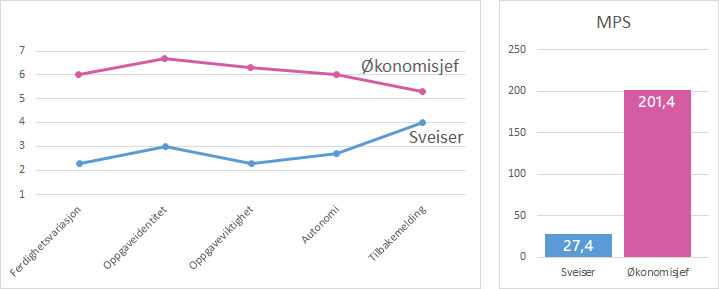
\includegraphics[width=135mm]{mps.png}
    \label{fig:mps}
\end{figure}
I figur \ref{fig:mps} ser vi en grov vurdering av motivasjonspotensialet til en sveiser og en økonomisjef i selskapet, basert på Hackman and Oldman’s Job Diagnostic Survey. Som vi ser, har økonomisjefen en mye høyere MPS (motivating potential score) enn sveiseren.


\subsection{Task B}
\subsubsection{Forslag til tiltak}
Vi vurderer jobbsituasjonen til økonomisjef Helle som god, men sveiserne sine jobber har forbedringspotensiale. Her kommer noen forslag til tiltak som kan øke sveisernes indre motivasjon, ytelse og jobbtilfredshet:

\begin{itemize}
  \item Ruller arbeidsoppgaver og la alle få delta på sluttmontering. Dette kan føre til høyere ferdighetsvariasjon, oppgaveidentitet, autonomi og tilbakemelding. Kort sagt får de brukt flere ferdigheter, får være med å bestemme hvordan ting blir gjort, de ser helheten av produktet og de kan få tilbakemelding om produktet fra kunden i sanntid.
  \item Flere besøk og samtaler mellom produksjonsavdelingen og ledelsen. La sveiserne ha regelmessige, korte møter med tegneren av maskinene som produseres. Da kan de føle at de får være med mer i diskusjonen av hvordan maskinene designes. De får altså mer oppgaveidentitet og autonomi.
\end{itemize}

Negative konsekvenser av forslagene kan være f.eks at mer rullering kan føre til mindre ekspertise på spesielle arbeidsoppgaver. Flere møter, besøk og samtaler kan føre til at mindre tid blir brukt på produksjon. Totalt sett kan dette føre til lavere kvalitet og effektivitet.
